\subsection{ソフトウェアテストツール}
テストは、多数の実行、結果の比較、大量の情報管理を伴うため、ツール支援が重要である。ツールは、単純な反復作業を減らし、テスト設計や生成を支援し、効率と有効性を高める。ただし、目的、開発方式、評価対象、実行環境に合うツールを選ぶ必要がある。一つの万能ツールではなく、複数のツールを組み合わせることが多い。

\subsubsection{テストツール支援と選択}
ツール選択では、何を自動化したいか、どの測度を集めたいか、どの環境で実行するか、既存プロセスとどう統合するかを確認する。ツール導入自体にも学習コスト、保守コスト、環境依存、誤判定、オラクルの限界がある。

\subsubsection{ツールの分類}
代表的なツール分類を表に示す。

\par\smallskip\noindent\refstepcounter{table}\label{tab:ch05-03}表 \thetable: ツールの分類の整理\par\smallskip
表 \thetable は、ツールの分類の整理を比較・確認しやすい形で整理したものである。\par\smallskip
\begin{longtable}{P{0.27\linewidth}P{0.63\linewidth}}
\toprule
分類 & 主な役割 \\
\midrule
テストハーネス & ドライバやスタブにより、部分的な SUT を制御された環境で実行し、出力を記録する。\\
テスト生成器 & ランダム、経路ベース、モデルベースなどによりテストケースを生成する。\\
キャプチャ・リプレイツール & 以前の入力や画面操作を記録し、再実行する。\\
オラクル・比較・表明検査ツール & 実行結果が成功かどうかの判定を支援する。\\
カバレッジ分析器・計測器 & プログラム中の文、分岐、経路などがどれだけ実行されたかを測る。\\
トレーサ & 実行経路の履歴を記録する。\\
回帰テストツール & 変更後の再実行、影響範囲に基づくテスト選択を支援する。\\
信頼性評価ツール & テスト結果を分析し、信頼性関連測度を可視化する。\\
注入ベースツール & 攻撃注入や欠陥注入により、特定条件での振る舞いを確認する。\\
シミュレーションベースツール & モデルを使ってシナリオを実行し、性質の検証や予測を行う。\\
セキュリティテストツール & 脆弱性、侵入、ファズテストなどを支援する。\\
テスト管理ツール & テスト計画、実行、データ収集、欠陥管理、報告を支援する。\\
クロスブラウザテストツール & 端末やブラウザごとに UI が期待どおり動くかを確認する。\\
負荷テストツール & 性能評価のために負荷を発生させ、関連データを集める。\\
欠陥追跡ツール & 欠陥報告、状態、修正履歴を管理する。\\
モバイルテストツール & 実機やエミュレータで、モバイルアプリの UI や動作を繰り返し確認する。\\
API テストツール & API の機能、性能、信頼性、セキュリティを自動テストする。\\
ウェブアプリケーションテストツール & ウェブベース SUT の機能、性能、利用者向け問題を確認する。\\
\bottomrule
\end{longtable}

\par\smallskip
\begin{center}
\centering
\IfFileExists{assets/generated_figures/ch05/fig-ch05-15.png}{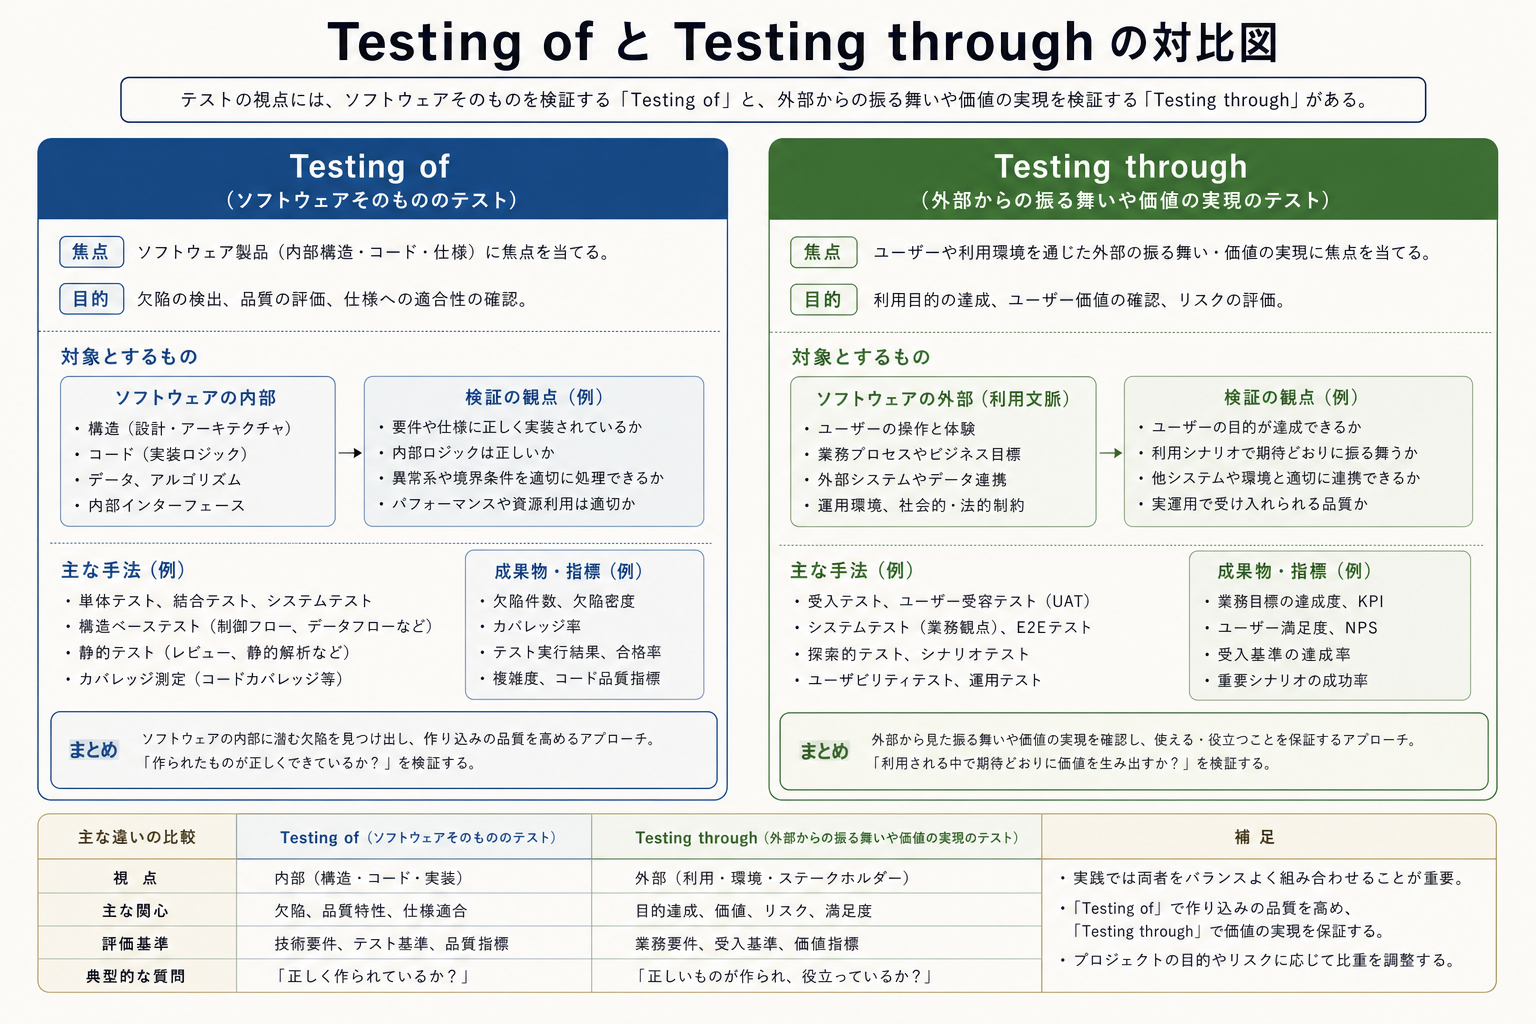
\includegraphics[width=0.96\linewidth]{assets/generated_figures/ch05/fig-ch05-15.png}}{\fbox{\parbox[c][48mm][c]{0.9\linewidth}{\centering 画像生成待ち\\テストツール分類図}}}
\par\smallskip
\refstepcounter{figure}\label{fig:ch05-15}図 \thefigure: テストツール分類図
\end{center}
図 \thefigure は、テストツール分類図を視覚的に整理したものである。
\par\smallskip
